\chapter{Proximal updates for online dictionary-learning}
\label{chap:proxdict}
\markright{{~{\rm \ref{chap:proxdict}}. Proximal updates for online dictionary-learning}\hfill}{}

\minitoc

\section{The power of the prox}
\newthought{Recall that after} $n$ passes over the data, the objective function whose minimization gives the dictionary updates is $E(\B{D}) := \frac{1}{2n}\|\B{X} - \B{D}\B{C}^T\|_{\text{F}}^2$, where $\B{C} \in \mathbb R^{n \times k}$ is the fixed matrix of codes computed up to this point, and $\B{D} \in \mathbb R^{p \times k}$ is the dictionary variable. Adding a \textbf{block-separable} penalty term $\gamma\sum_{j=1}^kg_j(\B{d}^j)$ the energy becomes
\begin{equation}
  E(\B{D}) = \frac{1}{2n}\|\B{X} - \B{D}\B{C}\|_{\text{F}}^2 + \gamma \sum_{j} g_j(\B{d}^j).
  \label{eq:model}
\end{equation}
One easily computes
$$\nabla_{\B{D}}\left(\frac{1}{2n}\|\B{X} - \B{D}\B{C}\|_{\text{F}}^2\right) = \frac{1}{n}(\B{DC} - \B{X})\B{C}^T = \B{DA} - \B{B},$$
where $ \B{A} := \frac{1}{n}\B{C}\B{C}^T = \frac{1}{n}\sum_{i=1}^n\B{c}_i\B{c}_i^T \in \mathbb R^{k \times k}$ and $\B{B} := \frac{1}{n}\B{X}\B{C}^T = \frac{1}{n}\sum_{i=1}^n\B{x}_i\B{c}_i^T \in \mathbb R^{p \times k}$. 
Now in BCD, the $j$th atom is updated whilst all the others are held constant. 
Selecting the $j$th column of \eqref{eq:model}, we get
$\nabla_{\B{d}^j}\left(\frac{1}{2n}\|\B{X} - \B{D}\B{C}\|_{\text{F}}^2\right) = \B{D}\B{a}^j - \B{b}^j$. Putting things together, we get
\begin{eqnarray*}
  \begin{split}
    &\B{p} = \argmin_{\B{d}^j \in \mathbb R^p,\;\B{d}^l\text{ fixed }\forall l \ne j}E(\B{D}) \iff
    \B{0} \in \partial_{\B{d}^j}E(\B{D}) = \B{D}\B{a}^j-\B{b}^j\big|_{\B{d}^j = \B{p}} + \gamma \partial g_j(\B{p})\\
    &\iff a_{j,j}\B{p} - \left(\B{b}^j-\sum_{l \ne j}a_{j,l}\B{d}^l\right) \in \gamma \partial (g_j)(\B{p})
    \overset{\text{Lemma} \ref{thm:implicit_grad}}{\iff} \B{p} = \prox_{\gamma a_{j,j}^{-1}g_j}(\B{z}^{-j})
\end{split}
\end{eqnarray*}
where
\[
  \B{z}^{-j} := a_{j,j}^{-1}\left(\B{b}^j-\sum\nolimits_{l \ne j}a_{j,l}\B{d}^l\right),
\]
and the last equivalence results from the following elementary lemma which reveals that the prox of a function at a point can be seen as an \textit{implicit} gradient step. Viz
\begin{lemma}
  For a function $f: \mathcal H \rightarrow (-\infty,+\infty]$ (convex or not), recall the definition of its \textit{subdiffferential} at a point $\B{p} \in \mathcal H$, namely  $\partial f(\B{p}) := \{\B{v} \in \mathcal H | f(\B{z}) \ge f(\B{p}) + \B{v}^T(\B{z} - \B{p})\; \forall \B{z} \in \mathcal H\}$. We have the following characterization of the prox
  \begin{equation}
    \B{p} \in \prox_{f}(\B{d}) \iff \B{d}-\B{p} \in \partial f(\B{p}).
\end{equation}

  \label{thm:implicit_grad}
\end{lemma}
\begin{proof}
  \[
    \begin{split}
      \B{p} \in \prox_{f}(\B{d}) &\iff \frac{1}{2}\|\B{p}-\B{d}\|_2^2 + f(\B{p}) \le \frac{1}{2}\|\B{z}-\B{d}\|_2^2 + f(\B{z})\; \forall \B{z}\\
      &\iff f(\B{p}) + \frac{1}{2}\|\B{p}\|_2^2 -\B{d}^T\B{p} \le f(\B{z}) + \frac{1}{2}\|\B{z}\|_2^2 -\B{d}^T\B{p}\; \forall \B{z}\\
      &\iff f(\B{p}) + \frac{1}{2}\|\B{p}\|_2^2 + \B{d}^T(\B{z}-\B{p}) \le f(\B{z}) + \frac{1}{2}\|\B{z}\|_2^2\;\forall \B{z}\\
      &\iff \B{d} \in \partial (f + \frac{1}{2}\|.\|_2^2)(\B{p}) = \B{p} + \partial f(\B{p})\\
      &\iff \B{d} - \B{p} \in \partial f(\B{p}).
    \end{split}
  \]
\end{proof}

% Recall that after $n$ passes over the data, the objective function whose minimization of which gives the dictionary updates is $E(\B{D}) := \frac{1}{2n}\|\B{X} - \B{U}\B{D}^T\|_{\text{F}}^2$, where $\B{U} \in \mathbb R^{n \times k}$ is the fixed matrix of codes computed up to this point, and $\B{D} \in \mathbb R^{p \times k}$ is the dictionary variable.
% A bit of algebra reveals that
% \[
% \begin{split}
%   E(\B{D}) &= \frac{1}{2n}\|\B{X} - \B{D}\B{U}\|_{\text{F}}^2 = \frac{1}{2n}\tr\left((\B{X} - \B{D}\B{U})^T(\B{X} - \B{D}\B{U})\right)
%    % + \frac{1}{2}\gamma\sum_{j=1}^k\|\K \B{d}^j\|_2^2
%    \\
%    &= \frac{1}{2n}\tr(\B{X}^T\B{X}) - \frac{1}{n}\tr(\B{X}^T\B{D}\B{U}) - \frac{1}{n}\tr(\B{U}^T\B{D}^T\B{X}) + \frac{1}{2n}\tr(\B{U}^T\B{D}^T\B{D}\B{U})\\
%    &= \frac{1}{2}\tr(\B{D}^T\B{D}\B{A}) - \tr(\B{D}^T\B{B}) + \frac{1}{2n}\tr(\B{X}^T\B{X}),
% \end{split}
% \]
% where $ \B{A} := \frac{1}{n}\B{U}\B{U}^T = \frac{1}{n}\sum_{i=1}^n\B{u}_i\B{u}_i^T \in \mathbb R^{k \times k}$ and $\B{B} := \frac{1}{n}\B{X}\B{U}^T = \frac{1}{n}\sum_{i=1}^n\B{x}_i\B{u}_i^T \in \mathbb R^{p \times k}$. Now, discarding the constant term $\frac{1}{2n}\tr(\B{X}^T\B{X})$ and simplifying, we get
% \[
%   \begin{split}
%  E(\B{D}) &= \frac{1}{2}\tr(\B{D}^T\B{D}\B{A}) - \tr(\B{D}^T\B{B}) = \sum_{j=1}^k\frac{1}{2}(\B{D}^T\B{D}\B{A})_{j,j} - (\B{D}^T\B{B})_{j,j}\\
%  &= \sum_{j=1}^k\frac{1}{2}\sum_{l=1}^ka_{j,l}\langle \B{d}^l,\B{d}^j\rangle - \langle \B{b}^j,\B{d}^j\rangle
%  = \sum_{j=1}^k\frac{1}{2}a_{j,j}\langle \B{d}^j,\B{d}^j\rangle - \left\langle \B{b}^j-\sum_{l \ne j}a_{j,l}\B{d}^l,\B{d}^j\right\rangle \\
%  &= \sum_{j=1}^k\tilde{E}_j(\B{d}^j) + \text{ stuff that don't depend on }\B{d}^j
%   \end{split}
% \]
% where $\tilde{E}_j(\B{z}) := \frac{1}{2}a_{j,j}\left\|\B{z} - a_{j,j}^{-1}\left(\B{b}^j-\sum_{l \ne j}a_{j,l}\B{d}^l\right)\right\|_2^2$, an expression which doesn't depend on any $\B{d}^l$ with $l \ne j$.

  
% \paragraph{Here comes the prox.}
% Now, if we consider a penalized version of the objective, namely $E(\B{D}) + \alpha R(\B{D})$, obtained by adding a \textbf{block-separable} penalty term $R(\B{D}) = \sum_{j=1}^kg_j(\B{d}^j)$, then each contribution $\tilde{E}_j(\B{d}^j)$ gets replaced by its penalized version $\tilde{E}_j(\B{d}^j) + \alpha g_j(\B{d}^j)$ and
% the BCD update for the $j$th atom is

% \begin{eqnarray}
%   \begin{split}
%     \B{d}^j \leftarrow \argmin_{\B{z} \in \mathbb R^p}\tilde{E}_j(\B{z}) + \alpha g_j(\B{z})
%     &= \argmin_{\B{z}  \in \mathbb R^p}\frac{1}{2}a_{j,j}\|\B{z} - a_{j,j}^{-1}\left(\B{b}^j-\sum\nolimits_{l \ne j}a_{j,l}\B{d}^l\right)\|_2^2 + \alpha g_j(\B{z})\\
%     &=:  \prox_{\alpha a_{j,j}^{-1}g_j}(\B{z}^{-j}),
%   \end{split}
% \end{eqnarray}
% where
% \[
%   \B{z}^{-j} := a_{j,j}^{-1}\left(\B{b}^j-\sum\nolimits_{l \ne j}a_{j,l}\B{d}^l\right).
% \]
% % \B{d}^j_{\text{old}} + a_{j,j}^{-1}(\B{b}^j-\B{D}\B{a}^j).$
Putting everything together, we have the close-form BCD update formula for regularized online dictionary learning\footnote{We assumed W.L.O.G that $a_{j,j} \ne 0$ (i.e $a_{j,j} > 0$), meaning that the $j$th atom is active in the representation of at least one sample. Otherwise, we can update the $j$th atom with a random vector, or even skip it altogether.}
\begin{shaded}
  \paragraph{BCD updates DL with general separable penalties.}
  The BCD updates for a penalized DL model \eqref{eq:model} is
\begin{equation}
  \B{d}^j \leftarrow \prox_{\gamma a_{j,j}^{-1}g_j}(\B{z}^{-j}),
\end{equation}
where $\B{z}^{-j} := a_{j,j}^{-1}\B{r}^j$ and $\B{R} := \left(\B{b}^j-\sum\nolimits_{l \ne j}a_{j,l}\B{d}^l\right) = \B{DA} - \B{B} + \B{d}^j \circ \B{a}^j $.
\end{shaded}

\paragraph{Convergence of the algorithm.}
Direct application of \cite{fercoq2015}, since the general DL algorithm constructs unbiased
estimates of $\nabla_j f(\B{D}_t)$, where $f(\B{D}) := \mathbb E_{\B{x}}\min_{\B{c} \in \mathbb R^k}\ell (\B{D}\B{c}, \B{x})$ ...

\section{Applications}
Now that we have the hammer, where are the nails...
\subsection{Special cases}
\subsubsection{Constraint sets}
If we take $g_j := i_{C_j}$, the indicator function of a closed convex subset of $\mathbb R^p$, so that each atom $\B{d}^j$ is constrained to satisfy a set of constraints prescribed by $C_j$, then the above updates reduce to projecting $\B{z}^{-j}$ onto $C_j$, namely
\begin{equation}
\B{d}^j \leftarrow  \text{proj}_{C_j}(\B{z}^{-j}).
\end{equation}
This is interesting as long as the $C_j$'s are sufficiently ``simple'' to allow us compute the above projection easily (preferably in closed form).
\paragraph{Classical choice.}

Taking $C_j$ to be $\mathbb B_2$, the unit ball for the euclidean norm on  $\mathbb R^p$, we recover the updates proposed in \citep{mairal2009,mairal2010}, namely
\begin{equation}
\B{d}^j \leftarrow  \frac{\B{z}^{-j}}{\max(1,\|\B{z}^{-j}\|_2)}.
\end{equation}
One notes that these constraint has no structural properties beyond preventing the dictionary atoms from becoming arbitrarily large.

\paragraph{Gram-Schmidt / step-wise orthonormality constraints.}
Akin to ICA-type methods, one can take $C_j =$ the orthogonal complement of the linear span of the first $j-1$st atoms, namely
  \begin{equation}
    C_{j} = \text{span}\{\B{d}^l | l < j\}^\perp \cap \mathbb B_{2}.
  \end{equation}
  The dictionary updates are then simply the Gram-Schmidt orthonormalization of the ordered sequence of vectors $\B{z}^{-1},\ldots,\B{z}^{-j}$, namely\footnote{The version of the Gram-Schmidt process presented here is not to be implemented as stated, as is it known to suffer from numerical instability errors in finite-precision arithmetic. There exists equivalent versions (e.g Golub \& Van Loan 1996] which alleviate these instabilities.\\}

  \begin{eqnarray}
    \tilde{\B{d}}^j \leftarrow \B{z}^{-j} -\sum_{l < j}\proj_{\B{d}^l}(\B{z}^{-j}),\;\B{d}^j \leftarrow \frac{\tilde{\B{d}}^j}{\|\tilde{\B{d}}^j\|_2},
  \end{eqnarray}
  where
  $$
  \proj_{\B{d}^l}(\B{z}^{-j}) := \begin{cases}\textbf{0},&\mbox{ if }\B{d}^l = \textbf{0},\\
    \frac{\langle \B{z}^{-j},\B{d}^l\rangle}{\langle \B{d}^l,\B{d}^l\rangle}\B{d}^l,&\mbox{ otherwise}
  \end{cases}
  $$
  is the orthogonal projection of $\B{z}^{-j}$ onto the line generated by the atom  $\B{d}^l$.
  

 \subsection{``Social'' sparsity:  simultaneous sparsity and smoothness via windowed group-Lasso}
The first non-trivial results of our ramblings this far is obtained by considering the \textit{social sparsity}  \citep{kowalski2013social,kowalski2009structured} prior. In this model, a weakly activated voxel $v$ in the middle of strongly activated voxels will be saved (as if rescued by the clan), whilst a strongly activated voxel in the middle of weakly activated voxels will be eliminated (as if killed by isolation). ``Strongness'' and ``weakness'' are measured with respect to a specified threshold $\alpha > 0$.
Formally, social sparsity corresponds to a penalty  $g_{\text{social}} : \mathbb R^p \rightarrow \mathbb R$ defined implicitly via its proximal operator

 \begin{marginfigure}
   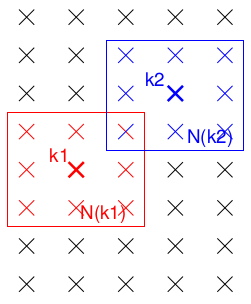
\includegraphics[width=\linewidth]{figures/social.png}
   \caption{\textbf{Social sparsity} illustrated in 2D. The neighborhood of the coefficient $k_1$ is given by the red
window, and the neighborhood of the coefficient $k_2$ by the blue one. These
two neighborhoods share one coefficient. When considering the red group,
coefficients are weighted by some weights $\boldsymbol{\gamma}_{k'}^{k_1} \ne 0$, $k' \in \mathcal N(k^1)$.
Outside the red group, the weights are equal to zero. When considering the blue group,
coefficients are weighted by some weights $\boldsymbol{\gamma}_{k'}^{k_2} \ne 0$, $k' \in \mathcal N(k^2)$.
Adapted from~\citep{kowalski2013social}.
}
\label{fig:social}
 \end{marginfigure}

 \begin{equation}
   \begin{split}
     (\prox_{\alpha g_{\text{social}}}(\B{z}))_v &:=
     z_v\begin{cases}1 - \frac{\alpha}{\|\boldsymbol{\gamma}_v \bullet \B{z}\|_2}, &\mbox{ if }\|\boldsymbol{\gamma}_v \bullet \B{z}\|_2 > \alpha
       % \text{ (i.e the average energy of neighbors of }v\text{ is high)}
       ,\\0, &\mbox{ otherwise}\end{cases}\\
     &=
     % z_v\left(1 - \frac{\alpha}{\|(\boldsymbol{\gamma}_v)^{1/2} \bullet \B{z}\|_2}\right)_+
     z_v\left(1 - \frac{\alpha}{\left(\sum_{s \in \mathcal N(v)}(\gamma^{s}_{v})^2z_{s}^2\right)^{1/2}}\right)_+, 
     \end{split}
  \label{eq:social}
\end{equation}
where $\boldsymbol{\gamma}_v \bullet \B{z} := (\gamma^1_v z_1,\gamma^2_v z_2,\ldots,\gamma^p_v z_p) \in \mathbb R^p$ for weights
$(\gamma^s_v)_{v,s \in [\![p]\!]}$ satisfying $\sum_v |\gamma^{s}_v|^2 = 1$ for all $s$, and $\mathcal N(v) := \{s \in [\![p]\!] | \gamma^{s}_v \ne 0\}$ is the \textit{neighborhood} of the $v$th voxel, assumed to be non-empty. Thus each $\boldsymbol{\gamma}_v$ can be thought of as
(normalized) mean-filter supported on a patch $\text{neigh}(v)$ around the voxel $v$.
Examples include rectangular filters, truncated Gaussians, etc.
%  Social sparsity applies a soft-thresholding using the norm of a local neighborhood, but modifies only the coordinate $\B{z}_v$ at the center voxel $v$ of this neighborhood.
%  It is a generalization of the overlapping group-lasso shrinkage operator\citep{ogrouplasso}; the latter is recovered by taking if the $w^v_s$ are chosen so that $w^v_s$ is independent of $s$ for all $s \in \text{neigh}(v)$, i.e $w^v_s = \frac{1}{\#\text{neigh}(v)}$ for all $v$ and $s \in \text{neigh}(v)$.
One notes the following facts
\begin{itemize}
\item $\|\B{E}\B{z}\|^2_2 \equiv \|\B{z}\|^2_2$, where $\B{E}\B{z} := (\boldsymbol{\gamma}_v \bullet \B{z})_{v \in [\![p]\!]} \in \mathbb R^{p^2}$
  is the \textit{expansion operator} associated with the weights $w^s_v$. In other words, $\B{E}$ is a \textit{linear isometry}.
\item social sparsity is related to GLasso by the formula
  \begin{equation}
    \text{prox}_{\alpha g_{\text{social}}} = \B{F} \circ \text{prox}_{\alpha \text{GL}} \circ \B{E},
  \end{equation}
  where $\B{F}$ is the right pseudo-inverse of $\B{E}$.
\end{itemize}

% \clearpage
\bibliographystyle{plainnat}
\bibliography{bib_all}
